\documentclass{beamer-control}
\usepackage{beamer-control-singlefile}
\INCLUDEONLY{Implementation}
\begin{document}
\CONCEPT{Implementation}

\begin{SUMMARY}
\begin{itemize}
\item Implementation considerations
\item Practical realisation
\end{itemize}
\vfill References:
\begin{itemize}
\item \astrom{§11.5}
\end{itemize}
\end{SUMMARY}



\SUBCONCEPT{Implentation considerations}

\begin{frame}{Filtering the derivative}
\begin{itemize}
\item In application of PID control, derivative action will have high gain for high-frequency signals
\item High-frequency measurement noise creates large variations in the output signals and hence large variations in the control signal
\item We must therefore filter the signal before calculating its derivative through using a low-pass filter by replacing $k_d s$ with
\[\frac{k_d s}{1+sT_f}\]
\item The time constant of the filter $T_f=\tfrac{T_d}{N}$ controls the strength of the filtering where $N$ is typically chosen to have a value $5\leq N \leq 20 $
\end{itemize}
\end{frame}


\begin{frame}{Setpoint weighting}
	\begin{itemize}
		\item PID controllers typically exhibit an initial peak in the control signal due to the derivative of the reference signal
		\item This peak can be avoided by having the proportional and derivative action acting only on the process output as in Figure 11.1 (b)
	\end{itemize}
\begin{figure}
	\centering
	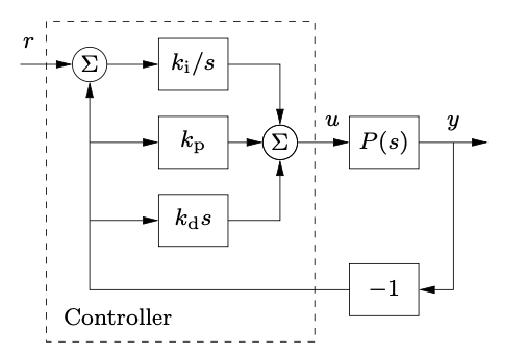
\includegraphics[width=0.6\linewidth]{figure11.1b}
	\\
	\textbf{Figure 11.1 (b):} Two degree-of-freedom PID controller. 
\end{figure}
\end{frame}

\begin{frame}{Setpoint weighting}
\begin{itemize}
	\item This form of PID controller is 
	\[u=k_p(\beta r - y) + k_i \int^t_0 \left( r(\tau)-y(\tau) \right) \, \mathrm{d} \tau + k_d\left(\gamma \frac{\mathrm{d}r}{\mathrm{d} t} -\frac{\mathrm{d}y}{\mathrm{d} t}\right)\]
	where the proportional and derivative actions act on fractions $\beta$ and $\gamma$ of the reference signal
	\item These parameters are known as the \textit{setpoint weights} and the resulting controller is called a two degree-of-freedom PID controller
	\item The response of the controller to a reference signal is dependent on $\beta$ and $\gamma$ but the response to load disturbances and measurement noise is the same
\end{itemize}
\end{frame}


\SUBCONCEPT{Practical realisation}

\begin{frame}{Analog implentation}
	\begin{itemize}
		\item PID controllers may be implemented in analog hardware using operational amplifiers 
		\item For the PI controller, $k_p=\tfrac{R_2}{R_1} $ and $k_i = \tfrac{1}{R_1C_2}$
		\item For the PID controller, $k_p = \tfrac{R_1C_1+R_2C_2}{R_1C_2}$, $T_i = R_1C_1+R_2+C_2$, and $T_d=\tfrac{R_1R_2C_1C_2}{R_1C_1+R_2C_2}$
	\end{itemize}
\begin{figure}
	\centering
	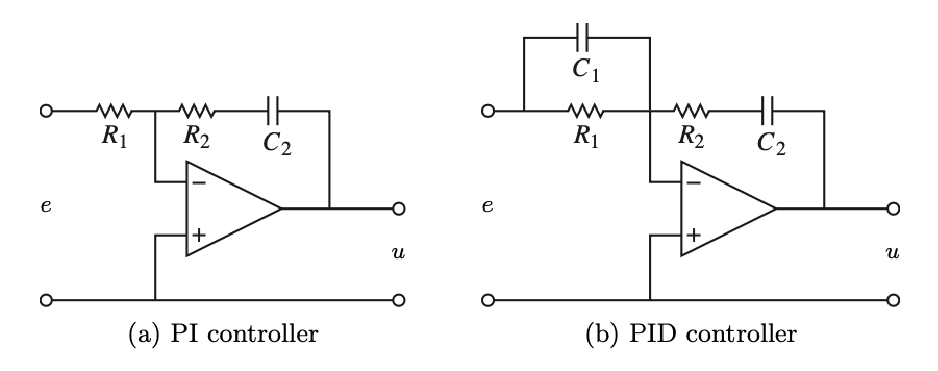
\includegraphics[width=0.8\linewidth]{figure11.14}
	\\
	\textbf{Figure 11.14:} Schematic diagrams for PI and PID controllers using op amps. 
\end{figure}
\end{frame}

\begin{frame}{Digital implentation}
\begin{itemize}
\item To implement a PID controller digitally onto a computer we must consider the process
\begin{enumerate}
	\item computer periodically samples the sensors
	\item convert the sensor signal to a digital form by an A/D converter
	\item compute the control signal 
	\item convert back to analog for the actuators
\end{enumerate} 
\item We therefore must approximate continuous-time systems as discrete-time systems
\end{itemize}
\end{frame}

\begin{frame}{Digital implementation}
	\begin{itemize}
		\item In discrete-time, the sampling instants (when the computer reads the input) are updated by the sampling time $h$ as $t_{k+1}=t_k+h$
		\item Considering the two degree-of-freedom PID controller, we can implement the proportional term by replacing $P=k_p(\beta r-y)$ with its sampled version
		\[P(t_k) = k_p (\beta r(t_k)-y(t_k))\]
		\item The integral term is found by approximating the integral with a sum
		\[I(t_{k+1}) = I(t_k)+k_i h e(t_k) + \tfrac{h}{T_{aw}} (\operatorname{sat}(u_a)-u_a)\]
		where $T_{aw}=h/k_{aw}$ represents the anti-windup term
	\end{itemize}
\end{frame}

\begin{frame}{Digital implementation}
	\begin{itemize}
		\item The filtered derivative term $D$ is found by the differential equation
		\[T_f \frac{\mathrm{d}D}{\mathrm{d} t} + D = -k_d \dot{y}\]
		\item Approximating the derivative with a backward difference gives
		\[D(t_k) = \frac{T_f}{T_f+h} D(t_{k-1})-\frac{k_d}{T_f+h}(y(t_k)-y(t_{k-1}))  \]
		\item This allows implementation onto PLCs or microcontrollers
	\end{itemize}
\end{frame}

\SUMMARYFRAME
\FINALE

\end{document}
